\documentclass[12pt]{article}
\usepackage[papersize={8cm,12cm},margin={.5cm,.5cm}]{geometry}
\usepackage{common}
\usepackage{amssymb}
\begin{document}
\begin{problem}
  \item[7.] 圖(三)中有一底面為直角三角形的直角柱 $ABCDEF$,其中 $\angle{BAC}$ 為直角。若 $\overline{AB} = 4$,$\overline{AC} = 3$,$\overline{AD} = 5$,則此三角柱的體積為何?
  \begin{figure}[ht]
    \centering
    \vspace*{-5ex}
    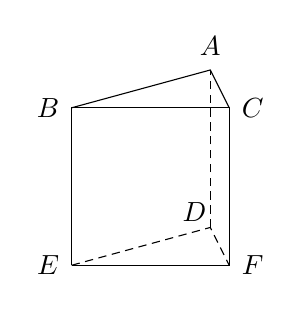
\begin{tikzpicture}
      \draw[densely dashed] (0,0) -- (1.76,.48) -- (2,0);
      \draw[densely dashed] (1.76,.48) -- (1.76,2.48);
      \draw (0,0) -- (0,2) -- (2,2) -- (2,0) -- (0,0);
      \draw (0,2) -- (1.76,2.48) -- (2,2);
      \node at (1.76,2.78) {$A$};
      \node at (-.3,2) {$B$};
      \node at (2.3,2) {$C$};
      \node at (1.56,.68) {$D$};
      \node at (-.3,0) {$E$};
      \node at (2.3,0) {$F$};
    \end{tikzpicture}
    \vspace*{-1ex}
    \caption*{圖(三)}
    \vspace*{-2ex}
  \end{figure}
  \begin{choices}
    \item 15
    \item 30
    \item 45
    \item 60
  \end{choices}
\end{problem}
\end{document}
